\documentclass{standalone}
\usepackage{tikz}
\usepackage{ctex,siunitx}
\setCJKmainfont{Noto Serif CJK SC}
\usepackage{tkz-euclide}
\usepackage{amsmath}
\usetikzlibrary{patterns, calc}
\usetikzlibrary {decorations.pathmorphing, decorations.pathreplacing, decorations.shapes,}

\begin{document}
\small
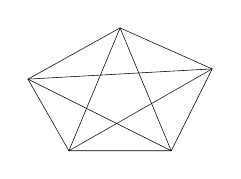
\begin{tikzpicture}[>=stealth,scale=1.3]
  \tkzSetUpPoint[fill=black]
  % \useasboundingbox(-1,-0.75)rectangle(3.7,1.4);
  \tkzDefPoints{0.2/0/A, 1.2/0/B, 1.6/.8/C,.7/1.2/D, -.2/.7/E}
  \tkzDrawPolygon(A,B,C,D,E)
  \tkzDrawSegments(A,C A,D B,D B,E C,E)
\end{tikzpicture}
\end{document}